\documentclass[a4paper]{article}
\linespread{1.6}
\usepackage{geometry}
\usepackage{setspace}
\usepackage{amsmath}
\usepackage{amssymb}
\usepackage{enumerate}
\usepackage{subfigure}
\usepackage{caption}
\usepackage{listings}
\usepackage{float}
\captionsetup{font = footnotesize}
\usepackage[pdftex]{graphicx}
\geometry{left=1cm,right=1cm,top=2.5cm,bottom=2.5cm}

\begin{document}
\begin{spacing}{2.0}
\begin{flushleft}\begin{huge}EEE6561  Fundamentals of Biometric Identification   Homework 5\end{huge}
\end{flushleft}
\begin{flushright}\begin{Large}Hudanyun Sheng\end{Large}\end{flushright}

\section*{\huge\textbf{ Task \uppercase\expandafter{\romannumeral1} Setup Environment and Download Code}  }
	\normalsize

	
\section*{\huge\textbf{ Task \uppercase\expandafter{\romannumeral2} Download and Enroll Iris Images}  }
	\normalsize

\section*{\huge\textbf{ Part \uppercase\expandafter{\romannumeral3} Matching}  }
	\normalsize

\section*{\huge\textbf{ Part \uppercase\expandafter{\romannumeral4} Analysis}  }
	\normalsize
	
	\begin{enumerate}
	\setcounter{enumi}{7}
	\item For the first three images in the probe set, the results of segmentation, noise masking, and iris coding is shown below:
	First image:\\
	
	\begin{figure}[H]
	\begin{minipage}[t]{0.3\linewidth}
	\centering
	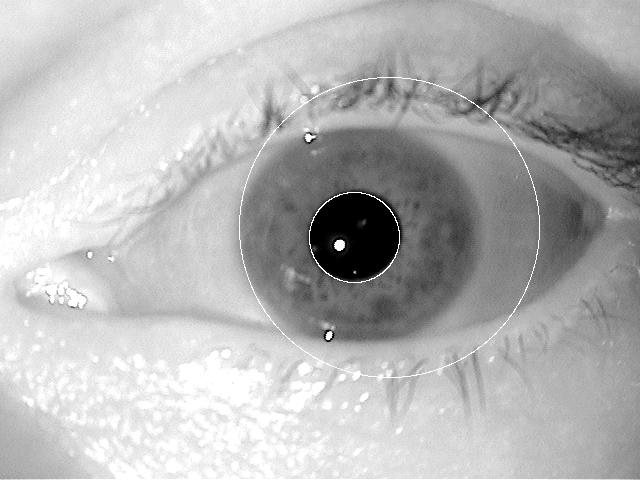
\includegraphics[width = 2.2in]{probe1segmented.jpg}
	\caption{The segmentation result of the 1st image.}
	\label{seg}
	\end{minipage}
	\begin{minipage}[t]{0.3\linewidth}
	\centering
	
\includegraphics[width = 2.2in]{probe1polarnoise.jpg}
	\caption{The noise masking result of the 1st image.}
	\label{noiseM}
	\end{minipage}
	\begin{minipage}[t]{0.3\linewidth}
	\centering
	
\includegraphics[width = 3in]{iriscoding1.jpg}
	\caption{The Iris coding result of the 1st image.}
	\label{IC}
	\end{minipage}
	\end{figure}
	
	Second image:\\
	
	\begin{figure}[H]
	\begin{minipage}[t]{0.3\linewidth}
	\centering
	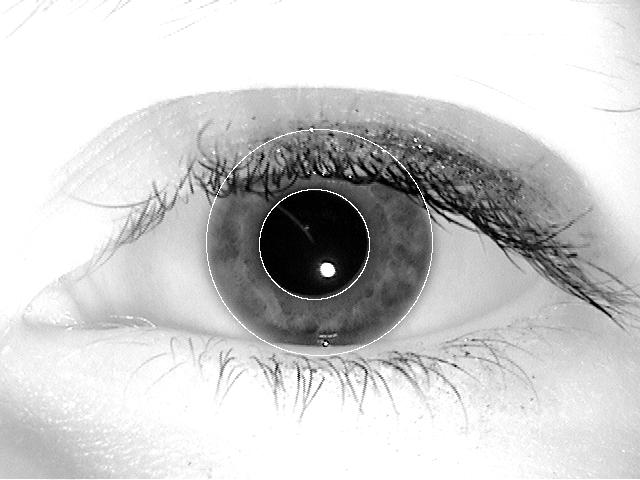
\includegraphics[width = 2.2in]{probe2segmented.jpg}
	\caption{The segmentation result of the 2nd image.}
	\label{seg}
	\end{minipage}
	\begin{minipage}[t]{0.3\linewidth}
	\centering
	
\includegraphics[width = 2.2in]{probe2polarnoise.jpg}
	\caption{The noise masking result of the 2nd image.}
	\label{noiseM}
	\end{minipage}
	\begin{minipage}[t]{0.3\linewidth}
	\centering
	
\includegraphics[width = 3in]{iriscoding2.jpg}
	\caption{The Iris coding result of the 2nd image.}
	\label{IC}
	\end{minipage}
	\end{figure}
	
	Third image:\\
	
	\begin{figure}[H]
	\begin{minipage}[t]{0.3\linewidth}
	\centering
	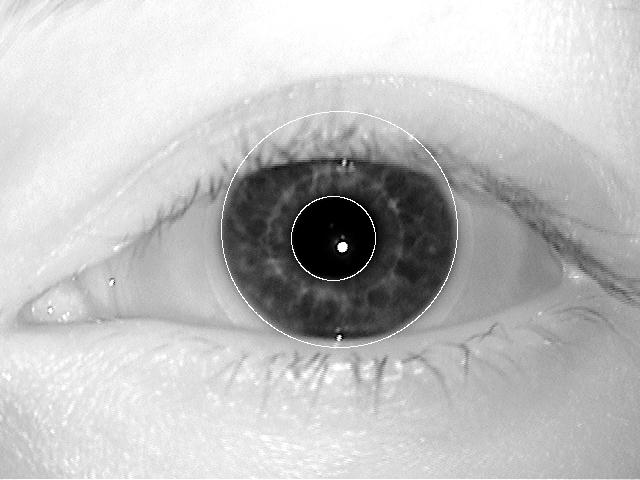
\includegraphics[width = 2.2in]{probe3segmented.jpg}
	\caption{The segmentation result of the 3rd image.}
	\label{seg}
	\end{minipage}
	\begin{minipage}[t]{0.3\linewidth}
	\centering
	
\includegraphics[width = 2.2in]{probe3polarnoise.jpg}
	\caption{The noise masking result of the 3rdimage.}
	\label{noiseM}
	\end{minipage}
	\begin{minipage}[t]{0.3\linewidth}
	\centering
	
\includegraphics[width = 3in]{iriscoding3.jpg}
	\caption{The Iris coding result of the 3rd image.}
	\label{IC}
	\end{minipage}
	\end{figure}
	
	
	\item  The values of mean and standard deviation of the genuine and imposter score distributions are shown below. We can see that the mean values of genuine and imposter scores differ no more than 0.2, and the standard deviation for the genuine distribution is about 7 times the imposter distribution. When looking at the d-prime value of the system, which measures the difference between two distributions, it is 3.3458.
	\begin{table}[H]
	\centering
	\begin{tabular}{lcc}
	\hline
	  & mean & standard deviation\\
	\hline
	genuine & 0.2898 & 0.0732 \\
	\hline
	imposter & 0.4668 & 0.0156\\
	\hline
	\end{tabular}
	\end{table}
	
	
	\item Two Gaussian distributions defines by the parameters calculated in question 9 is shown below:
	\begin{figure}[H]
	\centering
	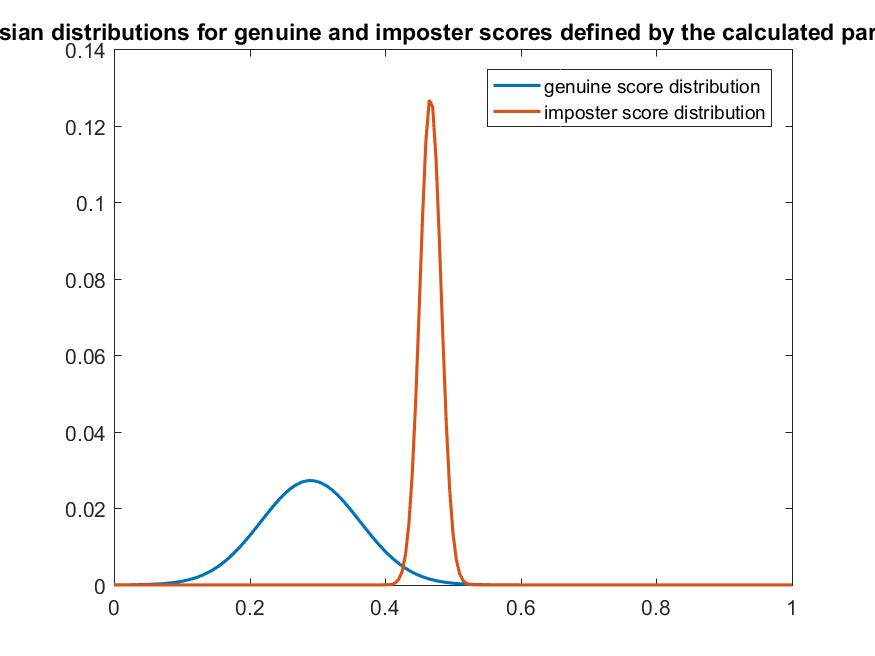
\includegraphics[width = 4in]{scoreDis.jpg}
	\end{figure}
	
	\item When examining the overlap of the distributions, I would consider this a set not easy to match. Although the center of the two distributions are separated, the variance of the genuine score is rather a big one, so that the overlap with the imposter score distribution is observed.
	
	\item The lowest scoring genuine pair of images is the 97th pair of probe and gallery images. As shown in figure \ref{probe97} and \ref{gallery97} below, the iris image from the probe set looks really similar to the iris image from the gallery set, they are both in good and similar illumination conditions, and both of them are really clear. The occlusion part of both of them are same. That is the reason they got a rather small distance score.
	\begin{figure}[H]
	\begin{minipage}[t]{0.5\linewidth}
	\centering
	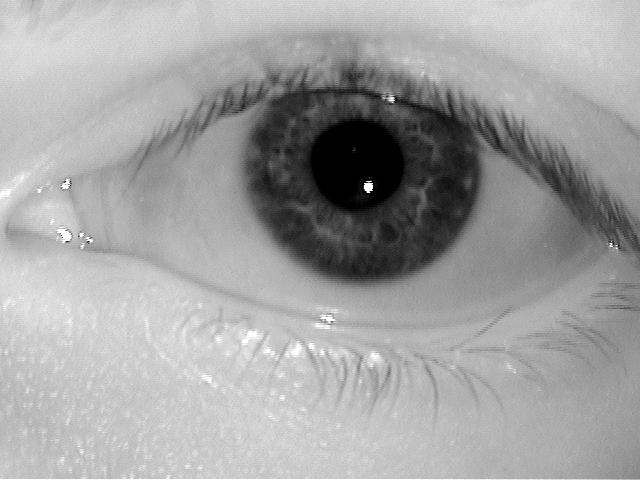
\includegraphics[width = 3in]{probe97.jpg}
	\caption{The 97th instance of the probe set.}
	\label{probe97}
	\end{minipage}
	\begin{minipage}[t]{0.5\linewidth}
	\centering
	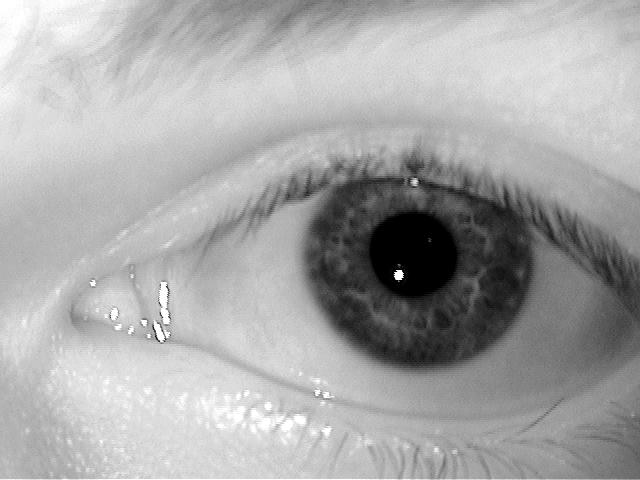
\includegraphics[width = 3in]{gallery97.jpg}
	\caption{The 97th instance of the gallery set.}
	\label{gallery97}
	\end{minipage}
	\end{figure}
	
	\item The highest scoring genuine pair of images is the 84th pair of probe and gallery image. As shown in figure \ref{probe84} and \ref{gallery84}, the images of the same instance from probe set and gallery set look really different. It is obvious that they are in different illumination conditions, and the instance from gallery set is obviously a blurred image with some occlusion compared to the one from the probe set. That is the reason they got a rather large distance score.
	\begin{figure}[H]
	\begin{minipage}[t]{0.5\linewidth}
	\centering
	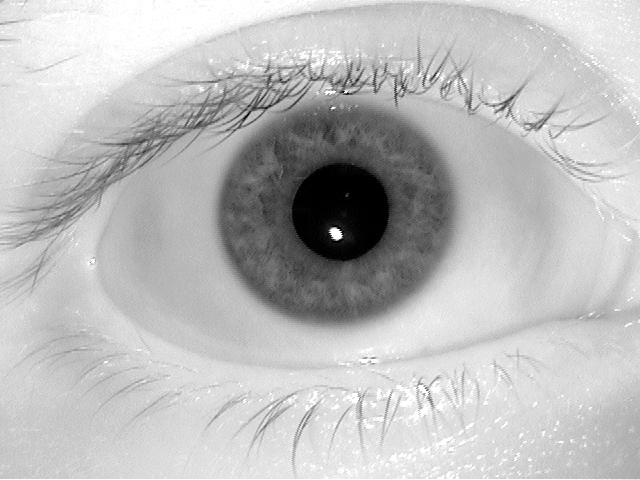
\includegraphics[width = 3in]{probe84.jpg}
	\caption{The 84th instance of the probe set.}
	\label{probe84}
	\end{minipage}
	\begin{minipage}[t]{0.5\linewidth}
	\centering
	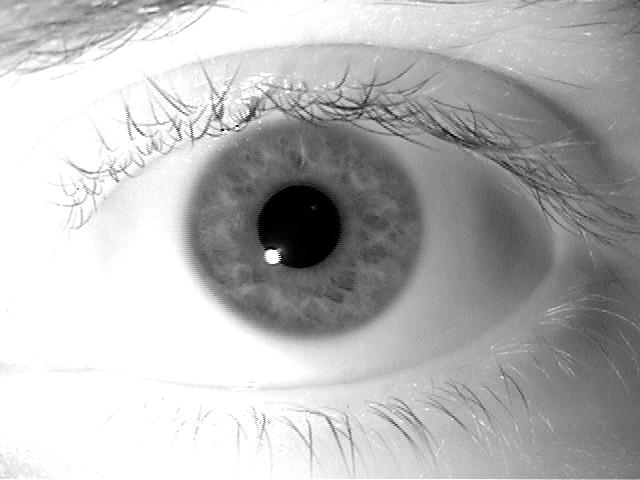
\includegraphics[width = 3in]{gallery84.jpg}
	\caption{The 84th instance of the gallery set.}
	\label{gallery84}
	\end{minipage}
	\end{figure}
	
	\item The lowest scoring imposter pair of images are 47th probe image matching 18th gallery image. As shown in figure \ref{probe47} and \ref{gallery18}, though from different instances, they are in similar good illumination condition. And they have really close occlusion. That is the reason they have lowest imposter distance score even if from different instances. 
	\begin{figure}[H]
	\begin{minipage}[t]{0.5\linewidth}
	\centering
	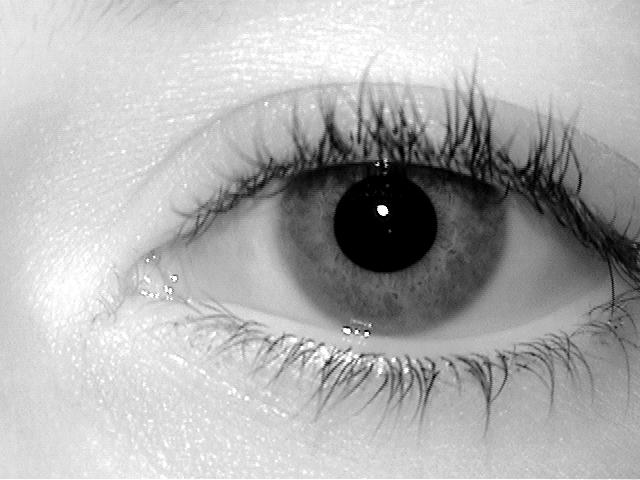
\includegraphics[width = 3in]{probe47.jpg}
	\caption{The 47th instance of the probe set.}
	\label{probe47}
	\end{minipage}
	\begin{minipage}[t]{0.5\linewidth}
	\centering
	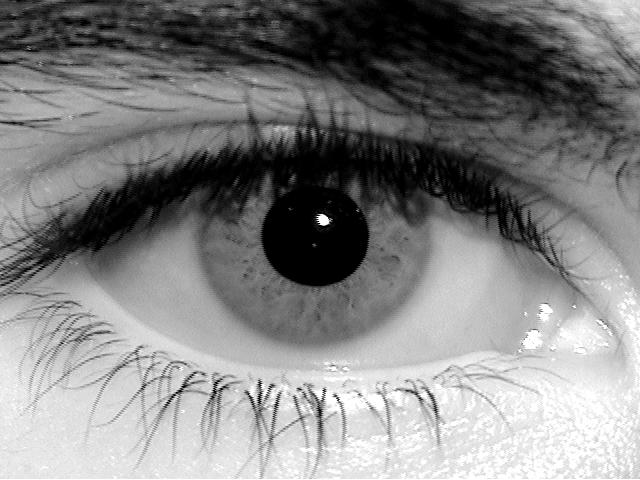
\includegraphics[width = 3in]{gallery18.jpg}
	\caption{The 18th instance of the gallery set.}
	\label{gallery18}
	\end{minipage}
	\end{figure}
	
	\item The highest scoring imposter pair of images are 45th probe image matching with 71st gallery image. As shown in figure \ref{probe45} and figure \ref{gallery71}, they are obvious from different instances, and what is more, they have different occlusion, different illumination condition, which will easily lead to highest distance scores.
	\begin{figure}[H]
	\begin{minipage}[t]{0.5\linewidth}
	\centering
	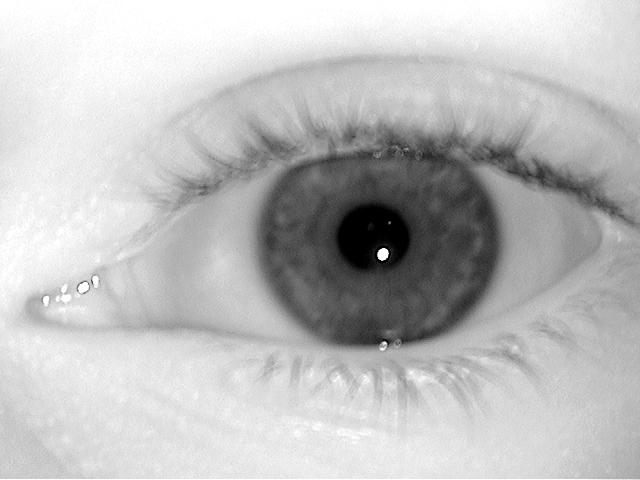
\includegraphics[width = 3in]{probe45.jpg}
	\caption{The 45th instance of the probe set.}
	\label{probe45}
	\end{minipage}
	\begin{minipage}[t]{0.5\linewidth}
	\centering
	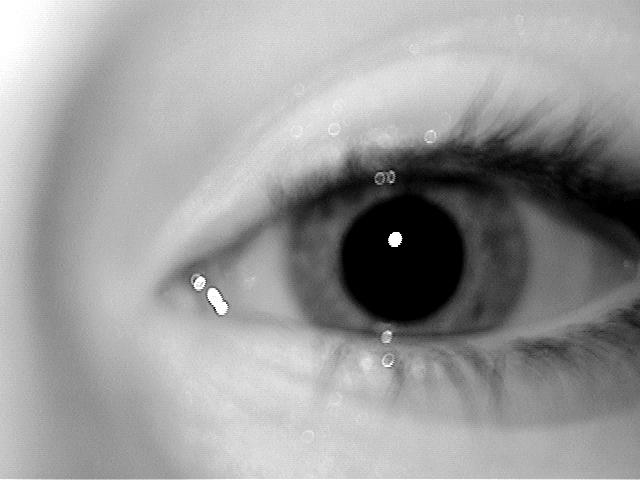
\includegraphics[width = 3in]{gallery71.jpg}
	\caption{The 71th instance of the gallery set.}
	\label{gallery71}
	\end{minipage}
	\end{figure}
	
	\end{enumerate}



\section*{\huge\textbf{ EXTRA CREDIT}  }
	\normalsize  With the images smoothed by a $5\times 5$ mean filter, the results are shown below:
	\begin{enumerate}
	\setcounter{enumi}{7}
	\item 	First image:\\
	
	\begin{figure}[h]
	\begin{minipage}[t]{0.3\linewidth}
	\centering
	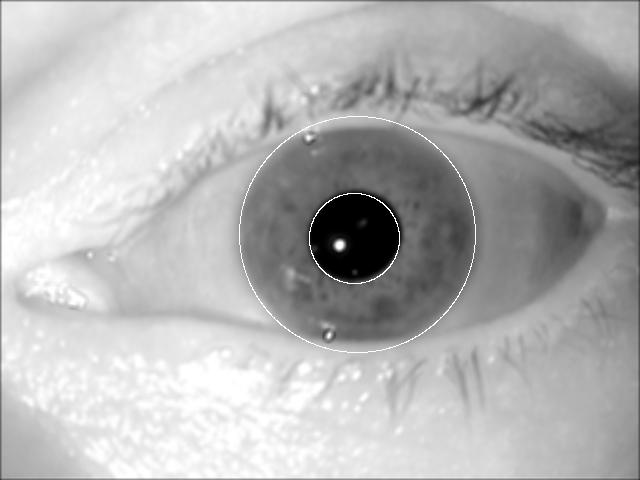
\includegraphics[width = 2.2in]{fprobe1segmented.jpg}
	\caption{The segmentation result of the 1st image.}
	\label{seg}
	\end{minipage}
	\begin{minipage}[t]{0.3\linewidth}
	\centering
	
\includegraphics[width = 2.2in]{fprobe1polarnoise.jpg}
	\caption{The noise masking result of the 1st image.}
	\label{noiseM}
	\end{minipage}
	\begin{minipage}[t]{0.3\linewidth}
	\centering
	
\includegraphics[width = 3in]{firiscoding1.jpg}
	\caption{The Iris coding result of the 1st image.}
	\label{IC}
	\end{minipage}
	\end{figure}
	
	Second image:\\
	
	\begin{figure}[H]
	\begin{minipage}[t]{0.3\linewidth}
	\centering
	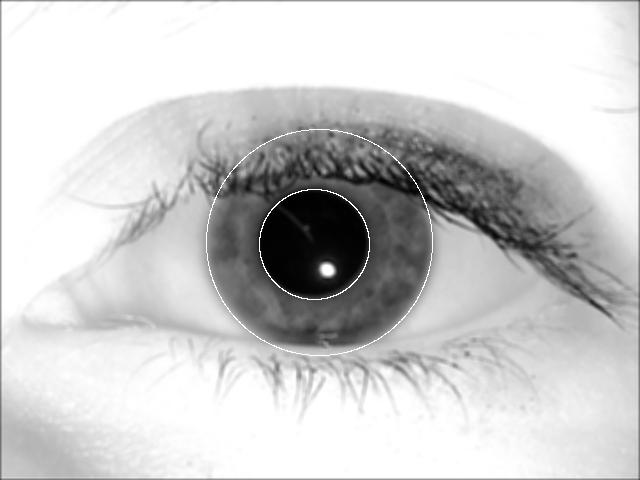
\includegraphics[width = 2.2in]{fprobe2segmented.jpg}
	\caption{The segmentation result of the 2nd image.}
	\label{seg}
	\end{minipage}
	\begin{minipage}[t]{0.3\linewidth}
	\centering
	
\includegraphics[width = 2.2in]{fprobe2polarnoise.jpg}
	\caption{The noise masking result of the 2nd image.}
	\label{noiseM}
	\end{minipage}
	\begin{minipage}[t]{0.3\linewidth}
	\centering
	
\includegraphics[width = 3in]{firiscoding2.jpg}
	\caption{The Iris coding result of the 2nd image.}
	\label{IC}
	\end{minipage}
	\end{figure}
	
		Third image:\\
	
	\begin{figure}[h]
	\begin{minipage}[t]{0.3\linewidth}
	\centering
	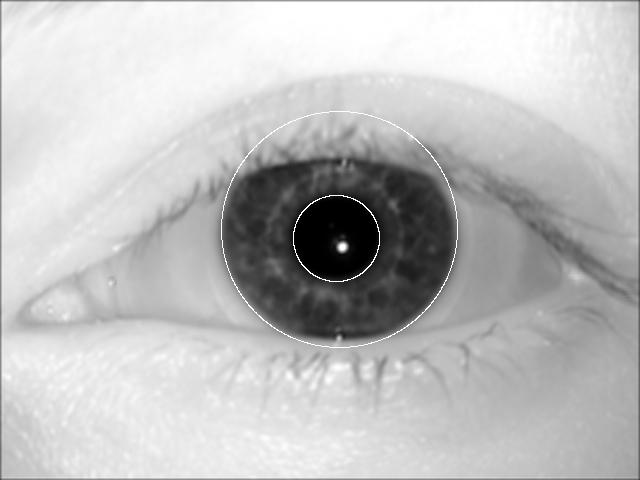
\includegraphics[width = 2.2in]{fprobe3segmented.jpg}
	\caption{The segmentation result of the 3rd image.}
	\label{seg}
	\end{minipage}
	\begin{minipage}[t]{0.3\linewidth}
	\centering
	
\includegraphics[width = 2.2in]{fprobe3polarnoise.jpg}
	\caption{The noise masking result of the 3rdimage.}
	\label{noiseM}
	\end{minipage}
	\begin{minipage}[t]{0.3\linewidth}
	\centering
	
\includegraphics[width = 3in]{firiscoding3.jpg}
	\caption{The Iris coding result of the 3rd image.}
	\label{IC}
	\end{minipage}
	\end{figure}
	
	
	\item The values of mean and standard deviation of the genuine and imposter score distributions are shown below. When looking at the d-prime value of the system, which implies the difference between two distributions, it is 3.3309. Compared to the former without smoothing, of which the d-prime value is 3.3458, it only becomes smaller a little bit.
	\begin{table}[H]
	\centering
	\begin{tabular}{lcc}
	\hline
	  & mean & standard deviation\\
	\hline
	genuine & 0.2781 & 0.0775\\
	\hline
	imposter & 0.4649 & 0.0169\\
	\hline
	\end{tabular}
	\end{table}
	
	\item Two Gaussian distributions defines by the parameters calculated in question 9 is shown below:
	\begin{figure}[H]
	\centering
	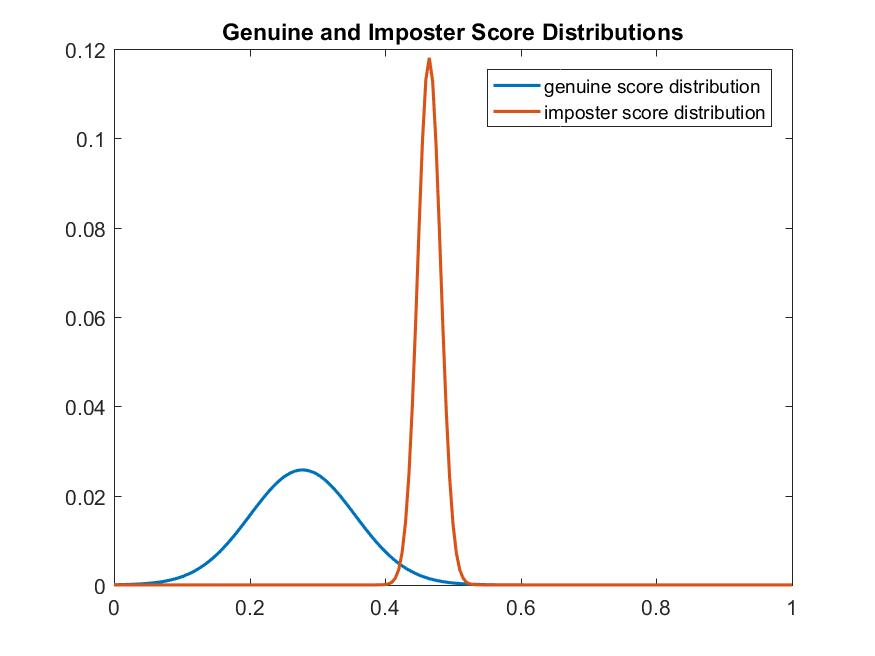
\includegraphics[width = 4in]{filtered_scoreDis.jpg}
	\end{figure}
	
	\item With examination of the overlap of the distributions, I would consider this an difficult set to match. Although the center of the two distributions are separated, the variance of the genuine score is rather a big one, so that the overlap with the imposter score distribution is observed.
	
	\item The lowest scoring genuine pair of images are 1st pair of images. As shown in figure \ref{probe1} and \ref{gallery1} below, the iris image from the probe set looks really similar to the iris image from the gallery set, they are both in good and similar illumination conditions, and both of them are really clear. The occlusion part of both of them are same. That is the reason they got a rather small distance score.
	\begin{figure}[H]
	\begin{minipage}[t]{0.5\linewidth}
	\centering
	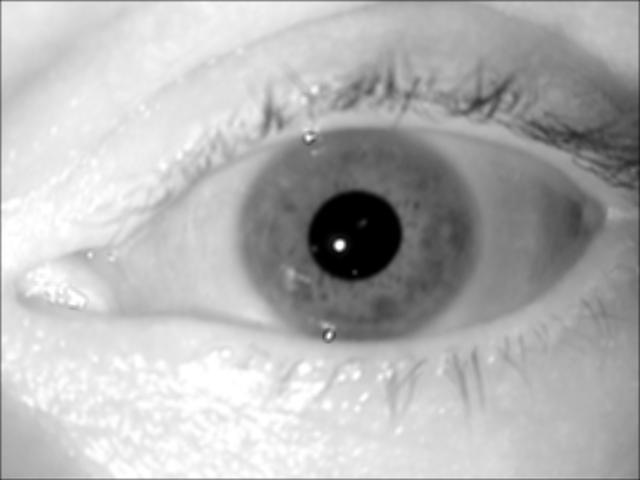
\includegraphics[width = 3in]{probe1.jpg}
	\caption{The 1st instance of the probe set.}
	\label{probe1}
	\end{minipage}
	\begin{minipage}[t]{0.5\linewidth}
	\centering
	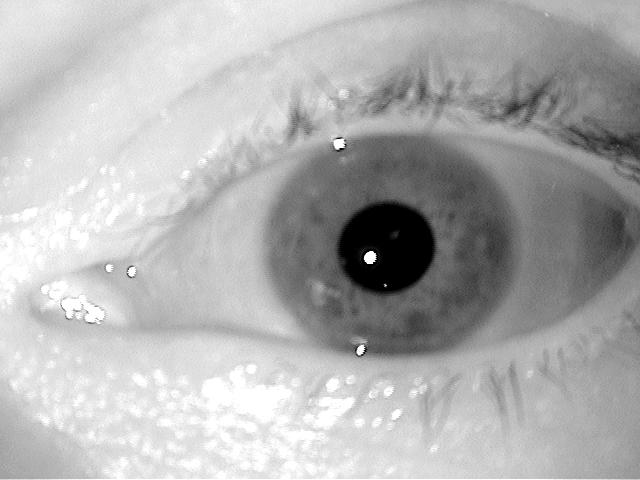
\includegraphics[width = 3in]{gallery1.jpg}
	\caption{The 1st instance of the gallery set.}
	\label{gallery1}
	\end{minipage}
	\end{figure}
	
	\item The highest scoring genuine pair of images is the 84th pair of probe and gallery image. As shown in figure \ref{probe} and \ref{gallery}, the images of the same instance from probe set and gallery set look really different. It is obvious that they are in different illumination conditions, and the instance from gallery set is obviously a blurred image with some occlusion compared to the one from the probe set. That is the reason they got a rather large distance score.
	\begin{figure}[H]
	\begin{minipage}[t]{0.5\linewidth}
	\centering
	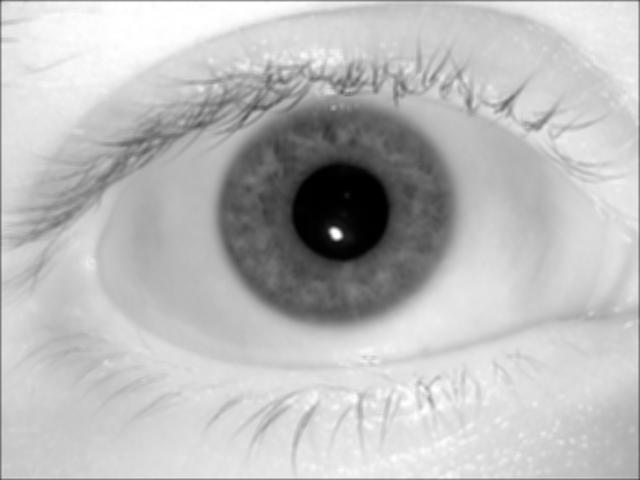
\includegraphics[width = 3in]{probe84filtered.jpg}
	\caption{The 84th instance of the probe set.}
	\label{probe}
	\end{minipage}
	\begin{minipage}[t]{0.5\linewidth}
	\centering
	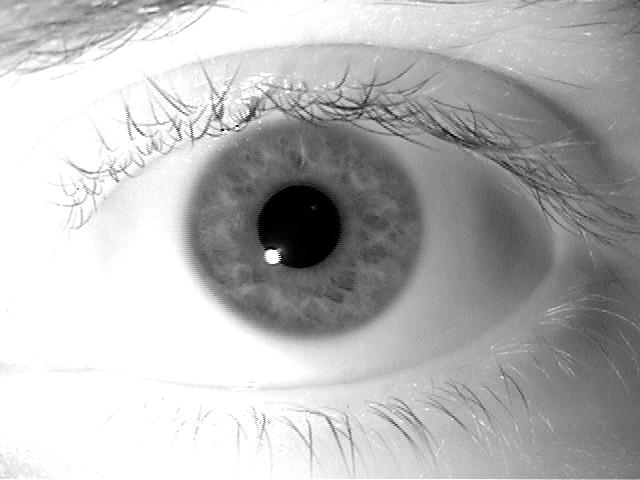
\includegraphics[width = 3in]{gallery84.jpg}
	\caption{The 84th instance of the gallery set.}
	\label{gallery}
	\end{minipage}
	\end{figure}
	
	\item The lowest scoring imposter pair of images are 66th probe image matching with 85th gallery image. As shown in figure \ref{probe66} and \ref{gallery85}, though from different instances, they are in similar good illumination condition. And they have really close occlusion. That is the reason they have lowest imposter distance score even if from different instances. 
	\begin{figure}[H]
	\begin{minipage}[t]{0.5\linewidth}
	\centering
	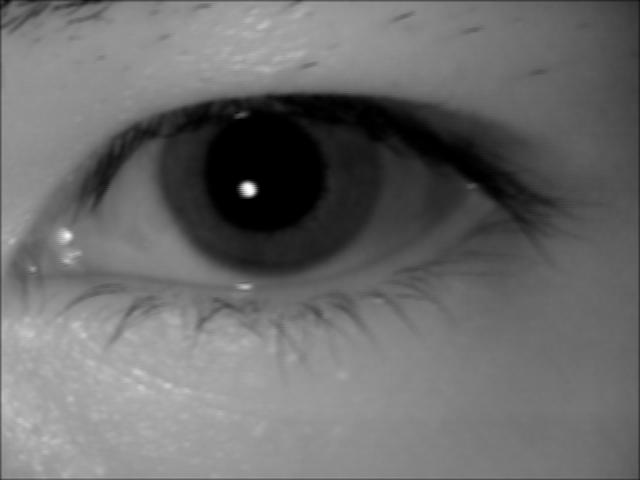
\includegraphics[width = 3in]{probe66filtered.jpg}
	\caption{The 66th instance of the probe set.}
	\label{probe66}
	\end{minipage}
	\begin{minipage}[t]{0.5\linewidth}
	\centering
	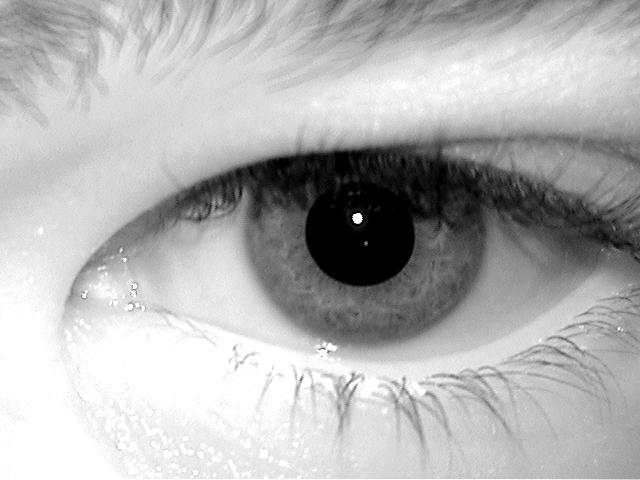
\includegraphics[width = 3in]{gallery85filtered.jpg}
	\caption{The 85th instance of the gallery set.}
	\label{gallery85}
	\end{minipage}
	\end{figure}

	
	\item The highest scoring imposter pair of images are 45th probe image matching with 71st gallery image. As shown in figure \ref{probe45f} and figure \ref{gallery71f}, they are obvious from different instances, and what is more, they have different occlusion, different illumination condition, which will easily lead to highest distance scores.
	\begin{figure}[H]
	\begin{minipage}[t]{0.5\linewidth}
	\centering
	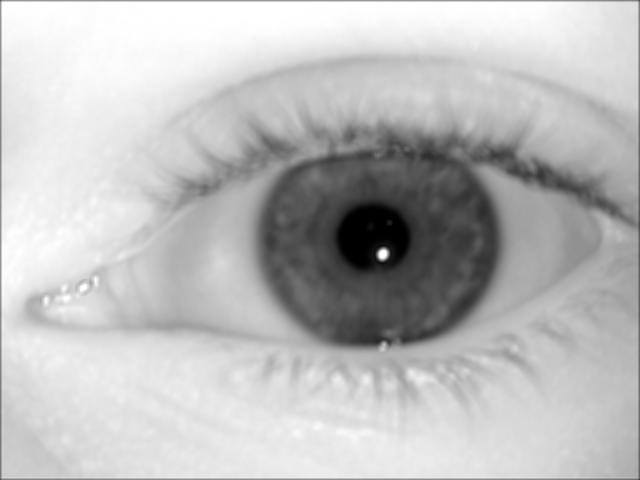
\includegraphics[width = 3in]{probe45filtered.jpg}
	\caption{The 45th instance of the probe set.}
	\label{probe45f}
	\end{minipage}
	\begin{minipage}[t]{0.5\linewidth}
	\centering
	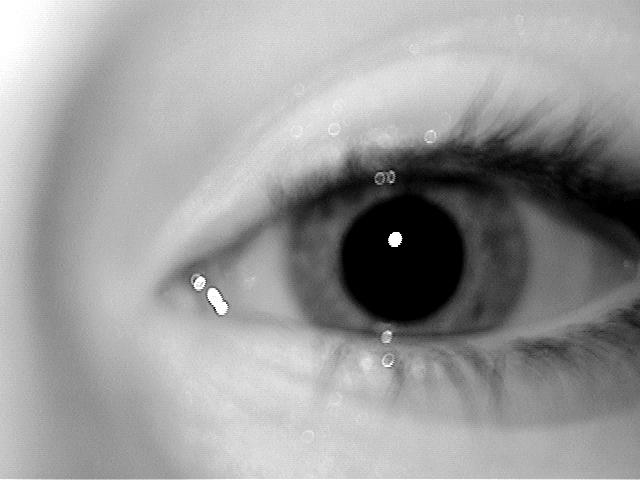
\includegraphics[width = 3in]{gallery71.jpg}
	\caption{The 71th instance of the gallery set.}
	\label{gallery71f}
	\end{minipage}
	\end{figure}
	
	\end{enumerate}
	
	Comment: compared to the results from the original data, there is no significant drop in matching performance when smoothing the probe images using a $5 \times 5$ mean filter. Some of the higher performing and lowest performing pairs using the blurred version of images are different. The reasons may be that smoothing procedure changes the impact of the original lighting conditions. When using the blurred version of the images, deblur can be used to improve the matching performance. 
	


	
\end{spacing}
\end{document}